\chapter{Generaci\'on de expresiones referenciales}

En este cap\'itulo daremos definiciones b\'asicas que nos servir\'an a lo largo de la tesis, en la Secci\'on \ref{sec:tipos_er} explicaremos los diferentes tipos de expresiones referenciales: las ER se diferencian seg\'un el tipo de propiedades que contengan, pueden contener propiedades at\'omicas, o relaciones con otros objetos, o ambas. Las ER tambi\'en se diferencian por la cantidad de informaci\'on que contienen, siendo las minimales las que alcanza para identificarlas, las sobreespecificadas contienen m\'as informaci\'on de la m\'inima necesaria para identificarlas, y las subespecificadas, las que no identifican a un target, sino a un conjunto m\'as grande el cual contiene al target y a otros elementos, por lo cual no se puede identificar al target. ER para plurales, son expresiones que identifican a un conjunto target, y las parciales, son las que siendo plurales, no alcanzan a identificar a todos los elementos del conjunto target. Luego en Secci\'on \ref{sec:tipos_algoritmos} explicaremos los diferentes tipos de algoritmos para la tarea de generaci\'on autom\'atica de ER: determin\'isticos son aquellos que dado un input fijo, siempre dan la misma ER, no-determin\'isticos son los que pueden dar distintas ER en 2 corridas del algoritmo con el mismo input, que generan sobreespecificaci\'on, que son los que pueden dar ER con m\'as de la m\'inima cantidad de informaci\'on que se necesita para identificar al target, plurales, son los que pueden dar ER para conjuntos de objetos, s\'olo singulares, son los que dan resultado s\'olo para un target singleton, relacionales o proposicionales, cuando pueden o no incluir relaciones y expresiones de los objetos relacionados. La Secci\'on \ref{sec:corpus2} est\'a dividida en 4 subsecciones, en las que nombramos las principales caracter\'isticas de corpora existente de ER dadas por humanos, como son el TUNA, el GRE3D3/7, el Stars y del ZOOM corpus, de \'este \'ultimo hablaremos sobre la obtenci\'on y daremos mucho m\'as detalle en el Cap\'itulo \ref{sec:corpus}, introducimos los corpus porque veremos que algunas aproximaciones emp\'iricas hacen uso de ellos. En la Secci\'on \ref{sec:algoritmos_area} contaremos la historia del \'area, y explicaremos los algoritmos m\'as conocidos como el incremental, GRAPH y bisimulaci\'on entre otros. En la Secci\'on \ref{sec:metricas_evaluacion} daremos una introducci\'on a las m\'etricas de evaluaci\'on en el \'area algunas que usan corpus para compararse y otras que no, algunas que necesitan jueces humanos y otras que son autom\'aticas.



\section{Generaci\'on {\emph humana} de expresiones referenciales}

Como usamos el lenguaje para trasmitir y entender intenciones? En la teor\'ia propuesta por (Clark 1992, Clark y Marshall 1981) una de las principales cosas que se cree es que el hablante usa un principio de dise\~no \'optimo, es decir, los hablantes dise\~nan sus oraciones de tal manera que sus interlocutores tengan suficiente informaci\'on para entenderles, pero no m\'as de la necesaria, hacen esto confiando en informaci\'on que ellos creen mutuamente que es parte del conocimiento mutuo, creencias mutuas y suposiciones mutuas. Y los oyentes conf\'ian en que van a recibir expresiones no ambiguas y concisas. 

En la investigaci\'on \cite{keysar:Curr98} han descubierto que bajo ciertas condiciones el hablante y el interloculor dejan de usar el principio de dise\~no \'optimo. %Cuando las personas conocen la motivaci\'on de un corportamiento ambiguo, lo ven menos ambiguo.
%Hubo gente (Sperber y Wilson 1982) que estuvo en contra del rol del conocimiento mutuo
Ellos compararon 2 modelos: 1 en el que el hablante sigue el principio de dise\~no \'optimo, planeando el mensaje teniendo en consideraci\'on la perspectiva del interlocutor, y otro en el que el dise\~no orientado al p\'ublico es m\'as bien una idea de \'ultimo momento, bajo este modelo de monitorear-ajustar los hablantes planean sus oraciones egoc\'entricamente sin importar la perspectiva de los interlocutores. Pero no son egoc\'entricos del todo, monitorean sus planes para detectar informaci\'on que no est\'a disponible al interlocutor.

Para testear estos modelos, le pidieron a los participantes dar una ER de un objeto en un contexto, pero a algunos participantes les dijeron que el interlocutor compart\'ia ese contexto, y a otros les dijeron que el interlocutor no pod\'ia ver esas figuras. Y quer\'ian ver cuando los hablantes confiaban en el contexto, lo cual fue indicado por adjetivos, por ejemplo, el c\'irculo peque\~no implica que hab\'ia por lo menos otro c\'irculo m\'as grande. Ah\'i se vi\'o que en ambos modelos la gente que sab\'ia que el interloculor compart\'ia el contexto, confi\'o en esa informaci\'on y lo que sugiere es que la descripci\'on final es sensitiva a la perspectiva del interlocutor (adhiriendo a la teor\'ia estandar). Otro test que hicieron, fue bajo presi\'on de tiempo, le pidieron a los participantes dar una expresi\'on 1,5 segundos luego de ver la figura, y las descripciones fueron como las que confiaban en que el interlocutor pod\'ia ver el contexto. Concluyen que bajo presi\'on los hablantes no tienen suficiente tiempo y recursos para monitorear y corregir sus oraciones y caen en el plan inicial, sus planes son egoc\'entricos en el sentido de que no tienen en cuenta el conocimiento mutuo con el interlocutor, el hablante conf\'ia en su propio contexto, m\'as all\'a que este no sea parte del conocimiento mutuo. As\'i como los hablantes planean sus oraciones egoc\'entricamente los oyentes interpretan esas oraciones desde su propia perspectiva egoc\'entrica, ellos no usan el conocimiento mutuo con el hablante a menos que sepan que est\'an en un error.


%\\
%\textcolor{blue}{ Esta parte, podria ir en algun lado donde ponga mas de discucion sobre sobreespecificacion junto con paper ivandre}
%\\

Normalmente las personas cuando hablan, dan m\'as informaci\'on de la m\'inima necesaria para identificar al target, a esto se le llama sobreespecificar y a las ER con m\'as informaci\'on de la m\'inima necesaria para identificarlas, sobreespecificadas. 

\cite{arts} estudiaron como las personas interpretan el lenguaje, 
hicieron experimentos sobreespecificando ER ya sea con informaci\'on de identificaci\'on relacionada con caracter\'isticas de los objetos (tama\~no, color, forma) o de ubicaci\'on (en el eje vertical u horizontal). Los resultados del experimento
proporcionaron informaci\'on sobre el efecto de la sobreespecificaci\'on en el tiempo de la identificaci\'on del target,
concluyen que las ER sobreespecificadas conducen a una identificaci\'on m\'as r\'apida del target, cuando permitieron que el lector 
tenga una imagen mental completa de la entidad, y que delimitan el comportamiento de b\'usqueda a una parte espec\'ifica
del contexto. La informaci\'on adicional sobre la ubicaci\'on vertical (arriba, abajo) ha demostrado ser
m\'as eficiente que la informaci\'on adicional sobre la ubicaci\'on horizontal (izquierda, derecha).

En \cite{do-speakers} tambi\'en se estudia la sobreespecificaci\'on, un experimento que realizaron mostr\'o que al menos la tercera parte de los hablantes sobreespecifica sus ER. Un segundo experimento mostr\'o que los oyentes no juzgan las descripciones sobreespecificadas de ser peores que las expresiones concisas. Y un tercer experimento en el que se utiliz\'o el paradigma de mundo visual para evaluar momento a momento a las interpretaciones por parte de los oyentes de los enunciados sobreespecificados, revel\'o que las descripciones sobreespecificadas desencadenan movimientos oculares que pueden interpretarse como una indicaci\'on de confusi\'on. Los resultados proporcionan apoyo para el uso de una simple heur\'istica como minimal o saturaci\'on con argumento.
%Llegan a la conclusi\'on de que las personas son s\'olo moderadamente \'optimas cuando generan expresiones.

%Nuestras observaciones verifican \'este hecho, y veremos m\'as adelante en este cap\'itulo que en un ejemplo de la Figura \ref{GRE3D7-stimulus} m\'as del 50\% de las ER dadas por personas fueron sobreespecificadas.

\cite{Lu_sasha2015} estudiaron el rol que la cantidad de informaci\'on juega en la adquisici\'on de nuevo vocabulario para un idioma extranjero en un entorno virtual. Experimentaron con 2 conjuntos de personas, a un conjunto se les dieron ER sobreespecificadas, y al otro minimales. Concluyeron que las ER sobreespecificadas ayudaron m\'as que las minimales a aprender palabras nuevas en idioma ruso.


%Los trabajos em\'iricos realizados en el \'area en la Secci\'on \ref{sec:trab_emp} explicaremos como trabaj\'o la gente usando corpora y las m\'etricas de evaluaci\'on en la Seccion \ref{sec:metricas_evaluacion} daremos una introducci\'on a los diferentes tipos de m\'etricas, autom\'aticas, manuales. 

 %(ver si los divido por secciones a los algoritmos...)
%ERORDENAR ESTO
%\cite{arec2:2008:Areces}~mostraron que el algoritmo de refinamiento utilizando el lenguaje de descripci\'on \el como lenguaje formal es capaz de generar 67\% de
%las ERs relacionales en el corpus ~\cite{viethen06:_algor_for_gener_refer_expres} cuando se consideran todos los posibles \'ordenes de las relaciones en el dominio. Esto est\'a en marcado contraste con el an\'alisis hecho en~\cite{viethen06:_algor_for_gener_refer_expres} sobre el cabinet corpus, de algoritmos basados en la propuesta original Dale y de Reiter.
%Los resultados de cobertura reportados sobre Viethen and 
%Dale's sobre el Cabinet corpus significan que~\emph{alg\'un orden} produce una razonablemente amplia cobertura. En otras palabras, se ha demostrado que los algoritmos de refinamiento tienen la capacidad de producir ERs similares a los producidos por los humanos, proporcionado una ordenaci\'on adecuada sobre las relaciones que aparecen
%en la escena de entrada, pero no est\'a claro cu\'al de todos los \'ordenes posibles se debe utilizar. En esta tesis abordamos directamente esta cuesti\'on.

%\section{Clasificaciones b\'asicas de ER y algoritmos GER}

%Esta secci\'on explicaremos los diferentes {\it tipos de ER}, as\'i como los diferentes {\it tipos de algoritmos} para generar algunos de los tipos de ER nombrados.

\section{Tipos de expresiones referenciales}
\label{sec:tipos_er}

Recordemos que en el Cap\'itulo \ref{sec:intro} dimos la definici\'on de \bf{expresi\'on referencial} (ER), dijimos que es un sintagma nominal que identifica a un target un\'ivocamente en un contexto dado para un interlocutor particular.

\begin{figure}[!ht]
\begin{minipage}[t]{0.5\linewidth}
\centering
\includegraphics[width=\textwidth]{images/22sinLetras.jpg}\\[0pt]
\caption{Contexto de una persona}
\label{GRE3D7-stimulus}
\vspace*{.1cm}
\end{minipage}
\hspace*{0cm}
\begin{minipage}[t]{0.5\linewidth}
\centering
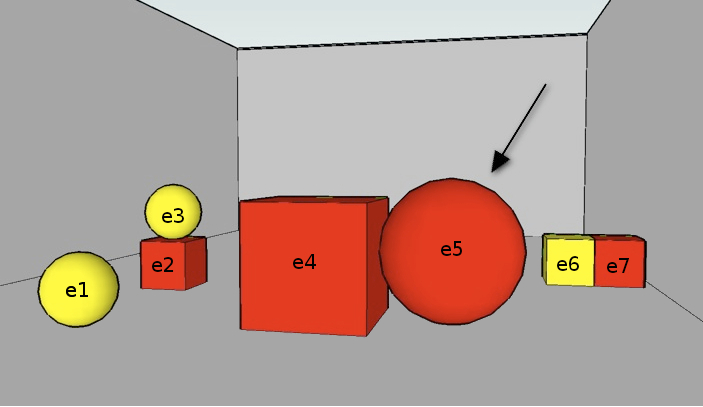
\includegraphics[width=\textwidth]{images/22.jpg}\\[0pt]
\caption{Contexto de un algoritmo}
\label{GRE3D7-stimulus-conLetras}
\end{minipage}
\end{figure}




Una propiedad es una caracter\'istica propia de un objeto. Por ejemplo en la Figura \ref{GRE3D7-stimulus} el objeto se\~nalado con la flecha tiene la propiedad {\it forma} con valor {\it esfera}. Por simplicidad, en el resto de la tesis vamos a decir ``tiene propiedad {\it esfera}'', cuando queremos decir que el objeto tiene la propiedad forma con valor esfera. Una relaci\'on caracteriza a un objeto describiendo caracter\'isticas de otro u otros objetos.

%Cuando la ER no es relacional solo contiene propiedades del objeto mismo. Ej.: color, tama\~no. Note que quiz\'as el tama\~no sea con respecto a los dem\'as objetos ``la m\'as peque\~na'', pero al no incluir una descripci\'on de otro objeto no la llamamos relacional.\\

De acuerdo a las propiedades o relaciones que una expresi\'on referencial incluya, se clasifican en distintos tipos: relacional o no relacional (tambi\'en llamada proposicional), minimal, sobreespecificada o subespecificada, plural o parcial. A continuaci\'on describimos cada uno de estos tipos.
% en cuyo caso es una expresi\'on que no es referencial, la incluimos en nuestras propiedades porque nos va a ser \'util la definici\'on en el Cap\'itulo \ref{sec:corpus}.\\
\begin{itemize}
\item Una ER {\bf proposicional} o no relacional, incluye s\'olo propiedades intr\'insecas del objeto target. Por ejemplo en la Figura \ref{GRE3D7-stimulus}: {\it La esfera roja}. Las caracter\'isticas de ser esfera, ser roja son propias del objeto identificado y no de su entorno.

\item Una ER es {\bf relacional}, cuando adem\'as de ser proposicional, contiene relaciones con otros objetos, entonces la ER incluye las descripciones de otros objetos con los cuales esta relacionada. Por ejemplo en la Figura \ref{GRE3D7-stimulus}: {\it La esfera que est\'a a la derecha del cubo}, {\it a la derecha de} lexicaliza una relaci\'on que necesita describir otro objeto adem\'as del target, en este caso {\it el cubo}.

\item \label{sec:minimales} Se dice que una ER es {\bf minimal}, cuando incluye la m\'inima cantidad de propiedades y/o relaciones con otros objetos, con las cuales el objeto puede ser distinguido en el contexto dado. Notar que puede haber muchas expresiones minimales. Por ejemplo en la Figura \ref{GRE3D7-stimulus} {\it La esfera roja} es una ER minimal, como as\'i tambi\'en lo es {\it La esfera grande}, o {\it La esfera a la derecha del cubo} ya que cada una de esas ER tienen propiedades que son necesarias para identificarlo. Para verificarlo intentemos sacar alguna propiedad, si de {\it La esfera roja} sacamos esfera, ya no tenemos al target, si sacamos roja, tampoco. Lo mismo pasa para {\it La esfera grande} no podemos sacar ni esfera ni grande. Veamos que pasa con {\it La esfera a la derecha del cubo}, si sacamos {\it esfera} tenemos otro objeto adem\'as del target que tambi\'en tiene a la izquierda un cubo, por lo tanto la expresi\'on no identificar\'ia al objeto.

\item Cuando la ER contiene m\'as informaci\'on de la m\'inima necesaria para distinguirlo de los dem\'as objetos en el contexto dado, se dice que la ER es {\bf sobreespecificada}. Por ejemplo: {\it La esfera roja grande} en la Figura \ref{GRE3D7-stimulus} es sobreespecificada porque se le puede sacar {\it grande} y sigue siendo ER, o se le puede sacar {\it roja} y tambi\'en sigue siendo ER.

\item Una expresi\'on es {\bf subespecificada} cuando no puede distinguir al target de los otros objetos en el contexto. Estos otros objetos son llamados {\it distractores}. Por ejemplo: {\it La esfera} en la Figura \ref{GRE3D7-stimulus} no alcanza para distinguir el objeto apuntado por la flecha, ya que hay otras 2 esferas. Una expresi\'on subespecificada identifica a un conjunto de objetos y ese conjunto incluye otros objetos adem\'as del target.

\item Una expresi\'on es {\bf plural} cuando el target agrupa varios objetos por ejemplo {\it Las esferas} es una ER para las 3 esferas de la Figura \ref{GRE3D7-stimulus}. Es interesante ver que {\it Las esferas} es una expresi\'on colectiva, pero otra ER para ese target podr\'ia ser {\it La esfera que est\'a sola, y la que esta arriba del cubo y la que est\'a al lado del cubo rojo}, la cual es una expresi\'on conjuntiva.

\item Una expresi\'on es {\bf parcial} cuando es una ER que representa parcialmente al target, en contextos plurales, por ejemplo la Figura \ref{GRE3D7-stimulus} si quisieramos identificar las 3 esferas y damos la expresi\'on {\it Las esferas peque\~nas}, es una expresi\'on que s\'olo identifica a 2 de las 3 esferas requeridas. Introducimos este concepto porque lo usaremos a lo largo de la tesis, en ejemplos plurales. 
\end{itemize}

\section{Psicoling\"u\'istica}

\section{Generaci\'on {\emph autom\'atica} de expresiones referenciales}
\label{sec:tipos_algoritmos}

Un algoritmo para la generaci\'on autom\'atica de expresiones referenciales es un programa que dado un input d\'a una ER para un target.

Los algoritmos pueden ser de distintos tipos, seg\'un los tipos de ER que sean capaces de generar. Los distintos tipos de algoritmos son: determin\'{i}stico o no-determin\'{i}stico, relacional o proposicional, incluir negaciones o no, generar plurales, singulares o ambos,
 %usar disyunciones y conjunciones, o s\'olo conjunciones, 
generar ER sobreespecificadas o minimales. A continuaci\'on se describen cada uno de esos tipos.

Un algoritmo es {\bf determin\'{i}stico} si dado un input (un contexto y un target), d\'a siempre la misma ER de salida. En cambio un algoritmo es {\bf no-determin\'{i}stico} si es posible que d\'e distintas salidas para el mismo input, en distintas ejecuciones. En general las personas generan expresiones referenciales de forma no determin\'istica, por lo tanto los algoritmos no-determin\'isticos simulan el comportamiento de distintas personas, o incluso el de la misma persona en distintos momentos. Por ejemplo ser\'ia no determin\'istico si para la Figura \ref{GRE3D7-stimulus-conLetras} una vez genera {\it La esfera roja} y otra vez {\it La esfera grande}. En la Tabla \ref{er-gre3d7-stimulus} se muestran las distintas ER dadas por las personas para la Figura \ref{GRE3D7-stimulus} y la cantidad de ocurrencias de cada ER en el corpus, por ejemplo {\it large red ball} ocurri\'o 71 veces en el corpus \cite{gre3d7}, el cual contiene 140 ER, si el algoritmo es determin\'istico dar\'ia s\'olo una ER. ?`Esa ER que dar\'ia el algoritmo coincidir\'a con alguna de las que dieron las personas?. 
Si el algoritmo es no-determin\'istico, ?`podremos conseguir todos los diferentes tipos de ER que dieron las personas?. %Intentaremos responder estas preguntas m\'as adelante en la tesis.\\
Si el largo de la ER es finito, dado un contexto finito, existen finitas ER a generar, as\'i un algoritmo no-determin\'istico nos permitir\'ia explorar todas las ER posibles para un input dado.

\begin{table}[h!]
\begin{center}
\begin{tabular}{|l|c|}
\hline
%total scenes in evaluation set &                           80   &             68
 ER& Cantidad \\
\hline
large red ball & 71 \\
red ball & 56 \\ 
large red ball next-to large red cube & 5 \\ 
large ball & 2 \\ 
large red ball next-to red cube & 2 \\ 
large red ball right-of large red cube & 1 \\ 
large red ball next-to large red ball & 1 \\ 
large red ball next-to cube & 1 \\ 
red ball next-to large red cube & 1 \\ \hline
Total & 140 \\ \hline
\end{tabular}
%\vspace*{.1cm}
\caption{ER dadas por las personas para la Figura \ref{GRE3D7-stimulus} del corpus GRE3D7.} 
\label{er-gre3d7-stimulus}
\vspace*{-.5cm}
\end{center}
\end{table}

Un algoritmo es {\bf proposicional}, cuando las ER que genera contienen s\'olo atributos del target, es decir no contiene relaciones con otros objetos ni expresiones de otros objetos. Por ejemplo para la Figura \ref{GRE3D7-stimulus2} {\it La esfera roja}. Genera ER proposicionales.

Un algoritmo es {\bf relacional} si adem\'as de generar ER proposicionales genera ER relacionales, en cuyo caso adem\'as de generar las relaciones correspondientes deber\'a generar expresiones para el o los objetos relacionados. Por ejemplo para la Figura \ref{GRE3D7-stimulus2} la ER {\it La esfera roja a la derecha del cubo}. En este caso {\it el cubo} es una expresi\'on que se tuvo que dar como consecuencia de incluir la relaci\'on {\it a la derecha de}. Notar que la expresi\'on {\it el cubo} no es una ER. En casos de generar ER relacionales hay que asegurarse que el algoritmo termina, es decir que no entra en loops tratando de identificar objetos. \cite{haddock} estudiaron como abordar el problema de regresi\'on infinita, en el cual el algoritmo trata de describir al landmark haciendo referencia al target, y al target haciendo referencia al landmark infinitamente, como en {\it el libro en la mesa la cual soporta un libro en la mesa... }

En algunos contextos cuando el target es el \'unico que no tiene una propiedad por ejemplo, ser\'ia \'util un algoritmo que incluya {\bf negaciones}. Por ejemplo para la Figura \ref{GRE3D7-stimulus}, si el target fuera $e_1$ la ER {\it La esfera que est\'a sola} podr\'ia ser sem\'anticamente equivalente a {\it la esfera que no est\'a tocando un cubo}.

Un algoritmo puede generar ER para {\bf plurales}, es decir dar ER para varios targets en el contexto considerado. Por ejemplo para la Figura \ref{GRE3D7-stimulus} la ER {\it Los cubos}. En este caso el target no es \'unico, sino un conjunto de objetos \{ $e_2$, $e_4$, $e_6$, $e_7$ \}. Estos algoritmos generan ER plurales.

Un algoritmo que genera ER {\bf minimales} las cuales se explicaron en la Secci\'on \ref{sec:minimales}, es un algoritmo que d\'a ER que contienen la m\'inima cantidad de propiedades o relaciones que se necesitan para distinguir al target.  Por ejemplo para la Figura \ref{GRE3D7-stimulus} {\it La esfera grande}. Notar que incluso puede haber varias ER minimales, como en este caso {\it La esfera roja}. Normalmente el orden de las propiedades hace que el algoritmo pueda decidir cual ER dar en caso de tener varias minimales.

Un algoritmo que haga {\bf sobreespecificaci\'on} tiene la caracter\'istica de poder dar m\'as atributos o relaciones de las m\'inimas necesarias para identificar al target. Por ejemplo para la Figura \ref{GRE3D7-stimulus} la ER {\it La esfera roja, grande que esta a la derecha del cubo rojo grande} es una ER sobreespecificada porque le podr\'iamos sacar {\it roja} o {\it grande} o y la relaci\'on con {\it el cubo rojo grande} y seguir\'ia siendo ER.

Notar que la ER con mayor frecuencia de la Tabla \ref{er-gre3d7-stimulus}, es una ER sobreespecificada, ya que {\it red ball} o {\it large ball}, eran algunos ejemplos minimales para el target de la Figura \ref{GRE3D7-stimulus}.

Para un algoritmo ser\'ia f\'acil hacer sobreespecificaci\'on simplemente podr\'ia agregar todas las propiedades y relaciones con todos los dem\'as obejtos que tiene y esa ser\'ia una ER sobreespecificada, pero esto no es lo que hace la gente, no sonar\'ia muy natural, por lo tanto lo que se estudia en esta tesis, es como hacer para el que el algoritmo sobreespecifique de cierto modo imitando el comportamiento humano lo m\'as posible. 

Los algoritmos no generan expresiones parciales ni subespecificadas, ya que ninguna de ellas es ER del target.








\section{Algoritmos importantes en el \'area}
\label{sec:algoritmos_area}
%interesante...
%https://www.abdn.ac.uk/ncs/departments/computing-science/tunabibl-495.php


En esta secci\'on vamos a hablar de los algoritmos de generaci\'on autom\'atica de expresiones referenciales, empezando por el algoritmo Full Brevity, siguiendo con el algoritmo de heur\'istica Greedy, luego Incremental, Graph, algoritmo Relacional y por \'ultimo Bisimulaci\'on. En la Tabla \ref{clasificacion_algoritmos} se muestra una clasificaci\'on seg\'un los tipos de algoritmos que vimos en la secci\'on anterior, siendo las columnas Det. - Determin\'istico, No-Det. - No-Determin\'istico, Prop. - Proposicional, Rel. - Relacional, Neg. - Genera Negaciones, Plur. - Genera Plurales, Sob. - Genera sobreespecificaci\'on. Notar que si no generan sobreespecificaci\'on, generan minimales. \\


\begin{table}[h!]
\begin{center}
\begin{tabular}{|l|c|c|c|c|c|c|c|}
\hline
%total scenes in evaluation set &                           80   &             68
 Algoritmos& Det. & No-Det. & Prop. & Rel. & Neg. & Plur. & Sob. \\
\hline
Full Brevity &Si & No&Si&No&No&No& No \\
Greedy&Si & No&Si&No&No&No& Si \\
Incremental&Si & No&Si&No&No&No& No \\
GRAPH&Si & No&Si&Si&No&Si& No \\
Bisimulaci\'on&Si & No&Si&Si&Si&Si& No \\ \hline
%Nuestra Propuesta&No & Si&Si&Si&No&Si& Si \\

\end{tabular}
%\vspace*{.1cm}
\caption{Clasificaci\'on de algoritmos seg\'un el tipo.} 
\label{clasificacion_algoritmos}
\vspace*{-.5cm}
\end{center}
\end{table}


 
%survey
%http://citeseerx.ist.psu.edu/viewdoc/download?doi=10.1.1.227.8284&rep=rep1&type=pdf

\subsection{Full brevity}

El algoritmo {\bf Full Brevity} \cite{Dale:1989:CUR:981623.981632} genera la descripci\'on m\'as corta que identifica al target. Para hacerlo, 
busca si hay una propiedad del target que no sea propiedad de ning\'un distractor. Si no hay chequea todas las posibles combinaciones de 2 propiedades, si no la hay, busca de a 3 y as\'i sucesivamente. Por ejemplo para la Figura \ref{GRE3D7-stimulus} se fijar\'ia en las propiedades del target {red, ball, large}, como ninguna de ellas aisladamente identifica s\'olo al target, probar\'ia con 2 propiedades {\it red ball} si identifica al target, devuelve {\it red ball} y finaliza.

\subsection{Heur\'istica Greedy}

Una aproximaci\'on a Full Brevity es el algoritmo de {\bf Heur\'istica Greedy}, el cual iterativamente selecciona la propiedad que elimina m\'as distractores y argumentan que la propiedad seleccionada tiene el m\'as alto poder discriminativo en esa etapa. Como resultado no siempre genera expresiones referenciales m\'inimas.

El problema es que encontrar la descripci\'on m\'as corta es computacionalmente caro, se observ\'o que las personas dan expresiones que no son minimales, esto fue confirmado por estudios psycoling\"uisticos \cite{Olson1970LangAndThought};  \cite{Sonnenschein1984}; \cite{Pechmann1989}; \cite{Engelhardt2006}.

El algoritmo de heur\'istica Greedy es m\'as eficiente que el Full Brevity, pero pronto fue superado por el algoritmo {\it Incremental} y sus sucesores \cite{C92-1038}; \cite{Dale95computationalinterpretations}. El algoritmo Incremental fue y sigue siendo uno de los algoritmos m\'as importantes del \'area, lo explicamos a continuaci\'on. Por ejemplo para la Figura \ref{GRE3D7-stimulus} se fijar\'a que {\it ball} elimina 2 distractores {$e_{1}$, $e_{3}$}, {\it red} elimina 3 distractores {$e_{2}$, $e_{4}$, $e_{7}$} y {\it large} elimina 1 distractores {$e_{4}$}, entonces elegir\'a {\it red}, pero como no alcanza para ser ER, seguir\'a con {\it ball} que es la que elimina m\'as distractores luego de {\it red}, finalizar\'a porque {\it red ball} identifica al target. Supongamos que hubiera otro objeto con propiedad {\it large}, entonces {\it large} eliminar\'ia tambi\'en 2 distractores, entonces el algoritmo devolver\'ia {\it large red ball}, y esa ER no es minimal, es sobreespecificada.

\subsection{Incremental}

\begin{figure}[ht]
%\centering
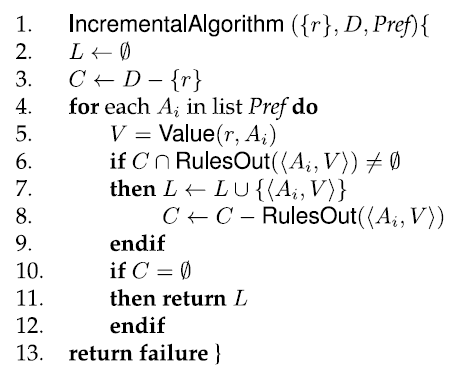
\includegraphics[width=0.5\textwidth]{images/algoritmoIncremental.png}
%\caption{Algoritmo Incremental}
\label{algoritmoIncremental}
\caption{Figura 2 de \protect\cite{survey}}
\end{figure}

%\begin{figure}[ht]
%%\centering
%\includegraphics[width=0.6\textwidth]{images/algIncremental.png}
%%\caption{Algoritmo Incremental}
%\label{algoritmoIncremental}
%\caption{Figura 2 de \protect\cite{survey}}
%\end{figure}

El input del {\bf Algoritmo Incremental}, es el target \emph{r}, que queremos identificar, $e_{5}$, \emph{D} es el dominio, y \emph{Pref} una lista de propiedades ordenada seg\'un la preferencia. Vamos a ejemplificar la corrida del algoritmo con el ejemplo de la Figura \ref{GRE3D7-stimulus-conLetras}, y supongamos que la lista ordenada de propiedades es \'esta [ tipo, color, tama\~no ]. \emph{D} inicialmente es el conjunto de todos los objetos del contexto: \{$e_{1}$,$e_{2}$,$e_{3}$,$e_{4}$,$e_{5}$,$e_{6}$,$e_{7}$\}.
En {\it Paso 2} se asigna a \emph{L} la descripci\'on vac\'{i}a, al finalizar la ejecuci\'on, \emph{L} tendr\'a el conjunto de propiedades con los cuales identificaremos a \emph{r}. Se inicializa \emph{C} con el conjunto de distractores de \emph{r} en nuestro ejemplo \{$e_{1}$,$e_{2}$,$e_{3}$,$e_{4}$,$e_{6}$,$e_{7}$\}, en el {\it Paso 3}. 
La idea del algoritmo es ir eliminando distractores, por eso, en el {\it Paso 4} recorre las propiedades $A_{i}$ de \emph{r}. En {\it Paso 5} le asigna a \emph{V} el valor que tiene la propiedad $A_{i}$ para el target \emph{r}, $RulesOut(A_{i},V)$ es el conjunto de objetos que tienen diferente valor para la propiedad $A_{i}$ que el que tiene el  target, la funci\'on se fija si el valor de esa propiedad elimina distractores. La primer propiedad de \emph{r} a considerar seg\'un el orden de preferencias \emph{Pref} es ``tipo'', el valor del target para tipo es {\it esfera}, entonces en {\it Paso 6}, pregunta si hay objetos en \emph{C} que tengan tipo con valor distinto de esfera, y hay, ellos son \{$e_{2}$,$e_{4}$,$e_{6}$,$e_{7}$\}, entonces le asigna a \emph{C} \{$e_{1}$,$e_{3}$\}, es decir s\'olo las que son esferas. En {\it Paso 10} pregunta si \emph{C} es vac\'io, es decir si ya se eliminaron todos los distractores, pero no lo es, por lo tanto continua con la siguiente propiedad, en este caso ``color'', el valor de color para el target es {\it rojo}, agrega {\it rojo} a \emph{L}, y actualiza \emph{C} con $\emptyset$ porque tanto $e_{1}$ como $e_{3}$ son amarillos, en {\it Paso 10} pregunta si \emph{C} es vac\'io, y si lo es, por lo tanto devuelve \{esfera, rojo\}. Lo cual se podr\'ia realizar como {\it La esfera roja}, y ser\'ia una ER para el target considerado.


\subsection{Algoritmo de b\'usqueda en Grafo}
\label{graph}

%\begin{figure}[ht]
%\centering
%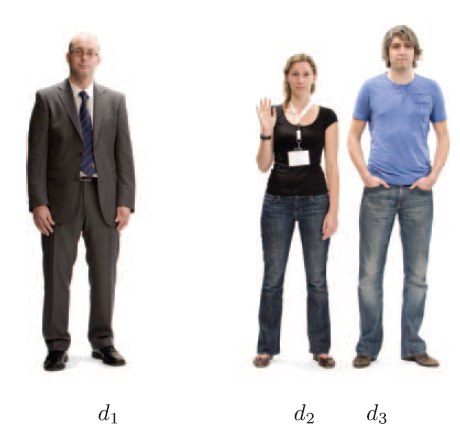
\includegraphics[width=0.4\textwidth]{images/contexto-survey.png}
%\caption{Ejemplo de contexto}
%\label{figura-survey}
%\end{figure}
%
%\begin{figure}[ht]
%\centering
%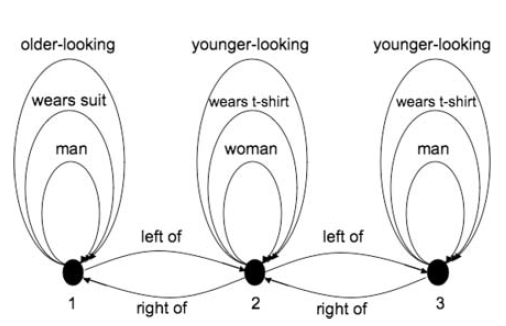
\includegraphics[width=0.4\textwidth]{images/grafo-survey.png}
%\caption{Ejemplo de grafo para el contexto de la Figura \ref{figura-survey}}
%\label{grafo-survey}
%\end{figure}





El {\bf algoritmo Graph} de \cite{Krahmer:2003} propone tratar la obtenci\'on de expresiones referenciales como un problema de grafos, el contexto que incluye al target y los distractores es representado como un grafo, por ejemplo para el contexto de la Figura \ref{figura-survey} el grafo correspondiente ser\'ia el de la Figura \ref{grafo-survey}. Cada objeto de la escena (personas en este caso) se modela como un v\'ertice en el grafo. Las propiedades at\'omicas como jounger-looking, older-looking, wears suit, wears t-shirt, woman, man, se representan como un bucle en el correspondiente nodo. Las relaciones binarias entre objetos, por ejemplo left-of o right-of se modelan como aristas entre los nodos correspondientes.

\begin{figure}[!ht]
\begin{minipage}[t]{0.4\linewidth}
\centering
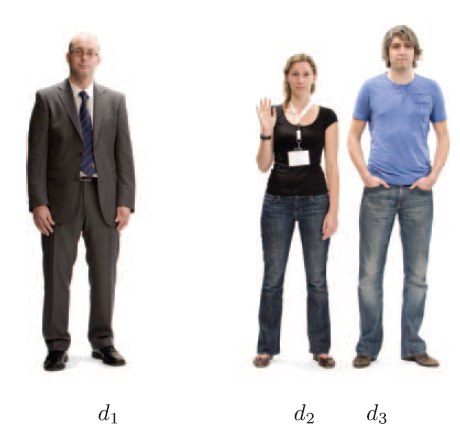
\includegraphics[width=\textwidth]{images/contexto-survey.png}\\[0pt]
\caption{Ejemplo de contexto}
\label{figura-survey}
\vspace*{.1cm}
\end{minipage}
\hspace*{0cm}
\begin{minipage}[t]{0.6\linewidth}
\centering
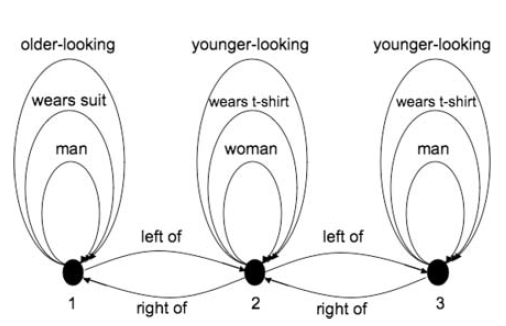
\includegraphics[width=\textwidth]{images/grafo-survey.png}\\[0pt]
\caption{Ejemplo de grafo para el contexto de la Figura \ref{figura-survey}}
\label{grafo-survey}
\end{minipage}
\end{figure}



Dado un objeto target, conseguir una ER que distinga al objeto de lo dem\'as es equivalente a encontrar un subgrafo del grafo original que unicamente caracterize al target. Intuitivamente este subgrafo se puede poner sobre el target y no sobre ningun otro objeto del dominio considerado.\\

\begin{figure}[ht]
\centering
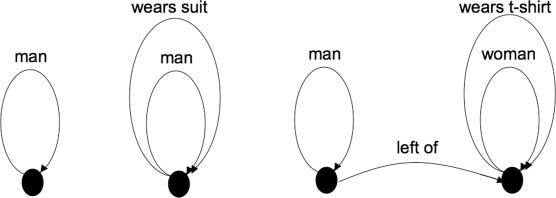
\includegraphics[width=0.6\textwidth]{images/ref-exp-graph.png}
\caption{Subgrafos de la Figura \ref{grafo-survey}}
\label{ref-exp-graph}
\end{figure}

%Para generar una descripci\'on distintiva, el algoritmo busca un subgrafo del grafo original que identifica al target un\'{i}vocamente al cual le llama grafo distintivo.% (distinguishing graph).\\
Comenzando con el subgrafo que contiene un solo v\'ertice, que representa al target, seg\'un una heur\'{i}stica basada en costos (costo de incluir propiedades, relaciones) empieza a agregar propiedades o relaciones, del target o nodos que ya hallan sido agregados. Cada vez que agrega algo, chequea si hay alg\'un otro nodo en el cual el grafo pueda distinguir, si lo hay quiere decir que es un distractor, cuando no hay el grafo distingue al target. Por ejemplo en la Figura \ref{ref-exp-graph} se ve el primer grafo {\it man}, el cual puede ser puesto sobre los nodos 1 y 3 de la Figura \ref{grafo-survey}, es decir no identifica s\'olo al target, el segundo grafo {\it man, wears suit} s\'olamente puede ser puesto sobre el nodo 1, por lo tanto es un grafo que distingue al target.  

El algoritmo sigue explorando grafos y siempre se queda con el de menor costo.

La funci\'on de costo esta definida sobre las aristas y v\'ertices del grafo dominio. El costo de un subgrafo se define como la suma sobre todas las aristas y v\'ertices que contiene el grafo.
El algoritmo de b\'usqueda garantiza encontrar el subgrafo de menor costo que representa al target.

La funci\'on de costo es usada para podar las ramas del \'arbol de b\'usqueda cuando estas se hacen m\'as costosas que el grafo de menor costo encontrado hasta el momento. Esta funci\'on hace que se prefieran propiedades sobre otras que tienen mayor costo.

%Por ejemplo, 
%Los algoritmos discutidos por Dale y Reiter (1995) pueden ser vistos como
%diferentes instancias de un algoritmo de b\'usqueda (Bohnet y Dale 2005; Gatt de 2007).
%Todos ellos, b\'asicamente, buscan a trav\'es de un mismo espacio de estados, compuestos por tres componentes: conjunto de cosas verdaderas para el target, un conjunto de distractores, y un conjunto de propiedades del target que a\'un no han sido consideradas. El estado inicial se puede formalizar como la tripla ($\emptyset$, C, P) 
%(no hay descripci\'on del target constru\'ida, no se han descartado distractores, y todas las propiedades P del target todav\'ia est\'an disponibles), y el estado final como
%(L, $\emptyset$, P'), se ha encontrado una descripci\'on que distingue al target,
%el conjunto de distractores est\'a vac\'io, y pueden o no quedar propiedades del target en P'. Todos los otros estados en el espacio de b\'usqueda son intermedios,
%a trav\'es de cuales un algoritmo podr\'ia moverse en funci\'on de su estrategia de b\'usqueda. 
%Por ejemplo 
%cuando buscamos de una descripci\'on distintiva de $e_{5}$ del Contexto\ref{GRE3D7-stimulus2}, un estado intermedio podr\'ia ser
%s = ({[forma, esfera],[color,rojo]},{$e_{5}$}, {[taman\~o, grande],[a-la-der-de, $e_4$]})
%
%Los algoritmos discutidos anteriormente difieren en el m\'etodo de creaci\'on de los estados, y en el orden en que estos estados son recorridos. Full Brevity, por ejemplo, utiliza un m\'etodo de expansi\'on, que crea un nuevo estado para cada atributo
%del target no contemplado antes (y que excluye al menos un distractor). 
%
%
%Comenzando desde el estado inicial y aplicando a nuestro ejemplo de contexto, este m\'etodo ser\'ia dar\'ia lugar a tres nuevos estados, la creaci\'on de descripciones, incluyendo la informaci\'on de forma, el color, y el taman\~o, respectivamente. Estos estados son chequeados mediante un m\'etodo de amplitud-primero. 
%El IA, por el contrario, utiliza un m\'etodo diferente para ampliar el grafo, cada vez que crea
%un nuevo estado, lo hace de acuerdo con un orden de preferencia predeterminado. As\'i, en
%el estado inicial, y suponiendo que (como antes) que escribe es el atributo m\'as preferido, el
%ampliar m\'etodo ser\'ia crear un solo nuevo estado: s = {[forma, esfera]}, siempre hay 1 solo nuevo estado elegido por el orden de preferencia.



\section{Corpus existente}
\label{sec:corpus2}
\label{sec:corpusTUNA}

%was the first prominent REG corpus to be made publicly available for research purposes. The corpus was developed in a series of general-purpose controlled experiments, containing 2280 descriptions produced by 60 speakers in two domains (1200 descriptions of furniture items and 1080 descriptions of people's photographs). TUNA does not contain relational descriptions, and it is possibly the only resource of this kind to include situations of reference to sets. The TUNA corpus has been extensively used in a series of shared tasks

{\bf TUNA} \cite{tuna-corpus} fue el primer corpus prominente para GER disponible p\'ublicamente con fines de investigaci\'on. El corpus fue desarrollado en una serie de experimentos controlados de prop\'osito general, contiene 2.280 descripciones producidas por 60 personas en dos dominios (1.200 expresiones referenciales de im\'agenes de muebles y 1080 expresiones referenciales de fotograf\'ias de personas situadas en una grilla). Se muestran ejemplos de im\'agenes en Figuras \ref{fig-TUNA-furniture} y \ref{fig-TUNA-people}. El corpus TUNA no contiene descripciones relacionales, y es posiblemente el \'unico recurso de este tipo que incluye situaciones de referencia a conjuntos. Este corpus se ha utilizado ampliamente en una serie de desaf\'ios \cite{reg2009}. 

\begin{figure}[!ht]
\begin{minipage}[c][][b]{0.5\textwidth}
%\begin{minipage}[H]{0.5\linewidth}
\centering
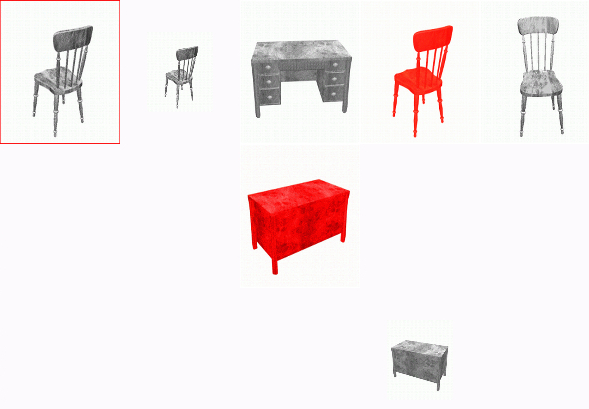
\includegraphics[width=\textwidth]{images/largeGreyChair.jpg}\\[0pt]
\caption{Imagen del TUNA corpus (muebles)}
\label{fig-TUNA-furniture}
\vspace*{.1cm}
\end{minipage}
\hspace*{0cm}
\begin{minipage}[c][][b]{0.5\textwidth}
%\begin{minipage}[H]{0.5\linewidth}
\centering
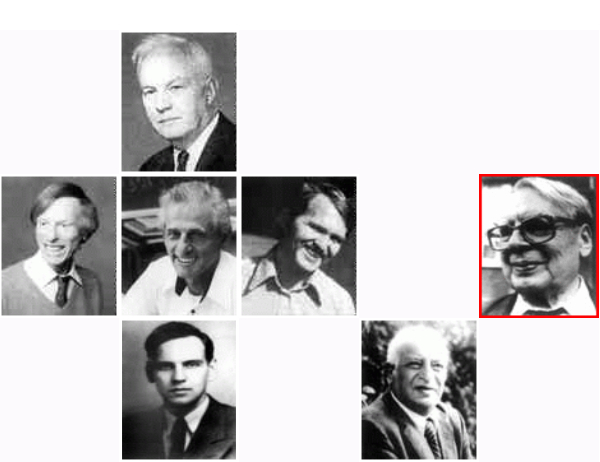
\includegraphics[width=\textwidth]{images/tuna-people.jpg}\\[0pt]
\caption{Imagen del TUNA corpus (personas)}
\label{fig-TUNA-people}
\end{minipage}
\end{figure}


\label{sec:corpusGRE}
%were developed in a series of web-based experiments primarily focussed on the study of relational descriptions. GRE3D3 contains 630 descriptions produced by 63 speakers, and GRE3D7 contains 4480 descriptions produced by 287 speakers, making it the largest of its kind to date. The GRE3D domain consists of simple visual scenes containing only two kinds of objects (boxes and spheres) with limited variation in colour and size. In each scene, there is only one possible spatial relation between target and the nearest landmark. Both corpora contain atomic and relational descriptions.
{\bf GRE3D3} y su extensi\'on {\bf GRE3D7} \cite{gre3d3,gre3d7} se desarrollaron en una serie de experimentos basados en la web, se centraron principalmente en el estudio de las descripciones relacionales. GRE3D3 contiene 630 descripciones producidas por 63 personas y GRE3D7 contiene 4.480 descripciones producidas por 287 personas, y es el corpus m\'as grande de este tipo hasta la fecha. El dominio del GRE3D3 consta de escenas visuales simples que contienen s\'olo dos tipos de objetos (cubos y esferas) con variaci\'on limitada en color y tama\~no. En cada escena, s\'olo hay una posible relaci\'on espacial entre el target y el landmark m\'as cercano. Ambos corpus contienen descripciones at\'omicas y relacionales. Ejemplo de im\'agenes del GRE3D3 y GRE3D7 se muestran en las Figuras \ref{fig-GRE3D3} y \ref{fig-GRE3D7}.
%\begin{minipage}[b]{0.45\linewidth}

\begin{figure}[!ht]
\begin{minipage}[b]{0.435\linewidth}
\centering
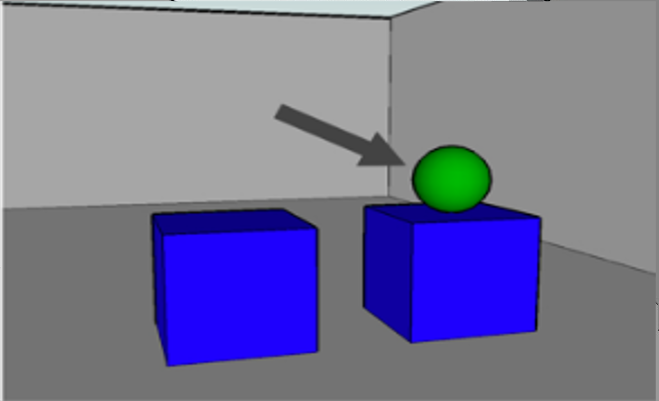
\includegraphics[width=\textwidth]{images/GRE3D3.png}\\[0pt]
\caption{Imagen del GRE3D3}
\label{fig-GRE3D3}
%\vspace*{-0.7cm}
\end{minipage}
\hspace*{0cm}
\begin{minipage}[b]{0.565\linewidth}
\centering
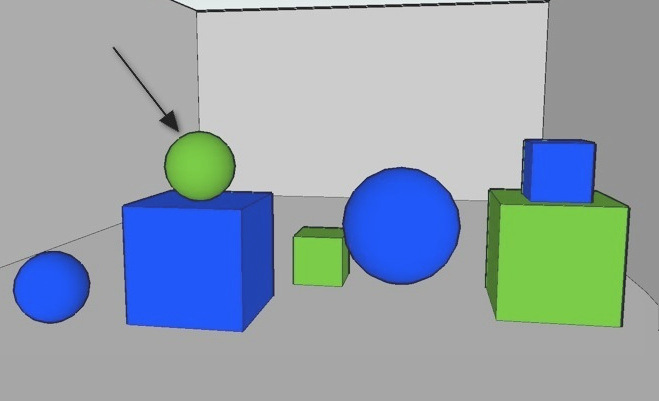
\includegraphics[width=\textwidth]{images/3.jpg}\\[0pt]
\caption{Imagen del GRE3D7}
\label{fig-GRE3D7}
\end{minipage}
\end{figure}

\vspace*{1cm}

\label{sec:corpusSTARS}
%and its extension Stars2 were collected for the study of referential overspecification (particularly in the case of relational descriptions). Stars was developed in a pilot web-based experiment, containing 704 descriptions produced by 64 speakers.  The more comprehensive Stars2 data set was produced in dialogue situations involving subject pairs, and it contains 884 descriptions produced by 56 speakers. Both domains make use of simple visual scenes containing up to four object types (e.g., stars, boxes, cones and spheres) with limited variation in colour and size. Differently from other REG corpora, however, Stars/2 includes a considerable number of complex situations of reference involving up to three objects, as in `the box near the sphere, next to the cone'.http://ppgsi.each.usp.br/arquivos/RelTec/PPgSI-002_2014.pdf y http://ppgsi.each.usp.br/arquivos/RelTec/PPgSI-001_2015.pdf
{\bf Stars} \cite{stars-mutual-disamb} y su extensi\'on {\bf Stars2} se recolectaron para el estudio de la sobre-especificaci\'on (particularmente en el caso de las descripciones relacionales). Stars se desarroll\'o en un experimento piloto basado en la web, contiene 704 descripciones producidas por 64 personas. El conjunto de datos Stars2 es m\'as completo y se obtuvo de situaciones de di\'alogo que implicaban a dos personas, contiene 884 descripciones producidas por 56 participantes. Ambos dominios hacen uso de escenas visuales simples que contienen tres tipos de objetos (por ejemplo para Stars, estrellas, cuadrados y c\'irculos y para Stars2 cubos, conos y esferas) con variaci\'on limitada en color y tama\~no. A diferencia de otros corpus para GER, Stars/2 incluyen un n\'umero considerable de situaciones complejas de referencia en que participan hasta tres objetos, como en {\it el cubo cerca de la esfera, al lado del cono}. Ejemplos de im\'agenes se muestran en las Figuras \ref{fig-STARS} y \ref{fig-STARS2}.

\begin{figure}[!ht]
\begin{minipage}[b]{0.5\linewidth}
\centering
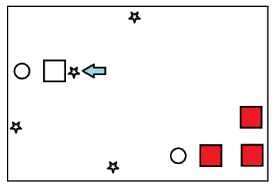
\includegraphics[width=\textwidth]{images/STARS.png}\\[0pt]
\caption{Imagen de Stars corpus}
\label{fig-STARS}
%\vspace*{1cm}
\end{minipage}
\hspace*{0cm}
\begin{minipage}[b]{0.5\linewidth}
\centering
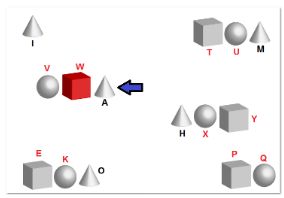
\includegraphics[width=\textwidth]{images/STARS2.png}\\[0pt]
\caption{Imagen de Stars2 corpus}
\label{fig-STARS2}
\end{minipage}
\end{figure}


\label{sec:corpusZOOM}
%were developed in a series of web-based experiments primarily focussed on the study of relational descriptions. GRE3D3 contains 630 descriptions produced by 63 speakers, and GRE3D7 contains 4480 descriptions produced by 287 speakers, making it the largest of its kind to date. The GRE3D domain consists of simple visual scenes containing only two kinds of objects (boxes and spheres) with limited variation in colour and size. In each scene, there is only one possible spatial relation between target and the nearest landmark. Both corpora contain atomic and relational descriptions.
El {\bf ZOOM} corpus se desarrollar\'o en un trabajo conjunto con la Universidad de S\~ao Paulo, contiene ER para 20 mapas de las ciudades de Lisboa y Madrid, fue realizado en la web, y contiene ER de targets singulares y plurales, con y sin zoom, en 2 idiomas: espa\~nol y portugu\'es. El corpus portugues contiene 100 ER por mapa, es decir 2000 ER en total, y el espa\~nol 80 por mapa, sumando un total de 1600 ER. El corpus fue recolectado a fin de poder hacer experimentos con situaciones mucho m\'as naturales que los corpus existentes hasta el momento. Ejemplos de esos mapas se muestran en las Figuras \ref{singularx}, \ref{singular2x}, \ref{pluralx}, \ref{plural2x}.


\begin{figure}[!ht]
\begin{minipage}[b]{0.46\linewidth}
\centering
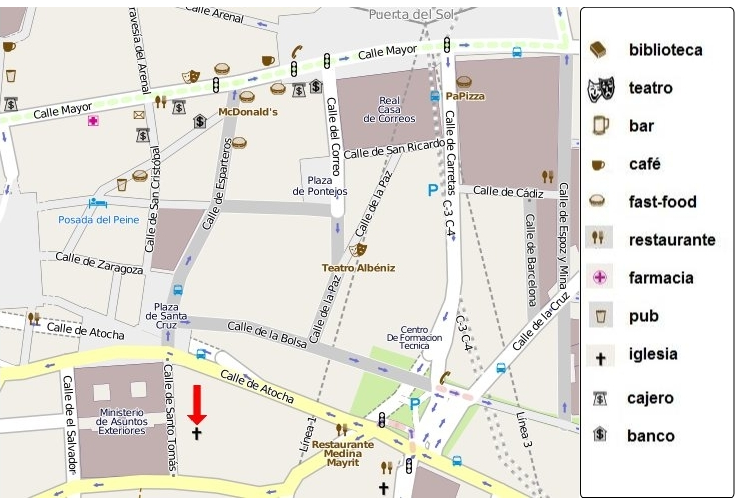
\includegraphics[width=\textwidth]{images/corpus/mapa6.png}\\[0pt]
\caption{Target singular con zoom X}
\label{singularx}
\end{minipage}
%\vspace*{.1cm}
\begin{minipage}[b]{0.54\linewidth}
\centering
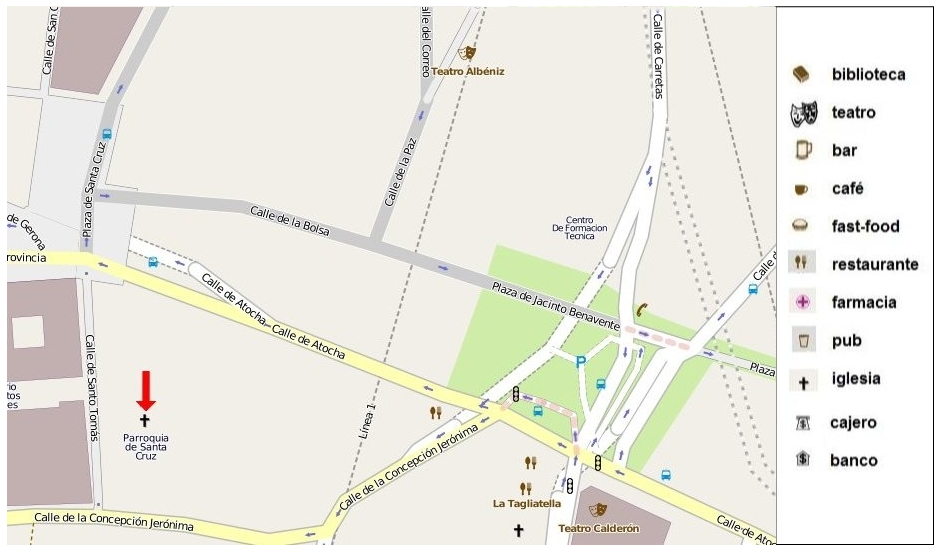
\includegraphics[width=\textwidth]{images/corpus/mapa16.png}\\[0pt]
\caption{Target singular con zoom 2X}
\label{singular2x}
\end{minipage}
\end{figure}

\begin{figure}[!ht]
\begin{minipage}[b]{0.47\linewidth}
\centering
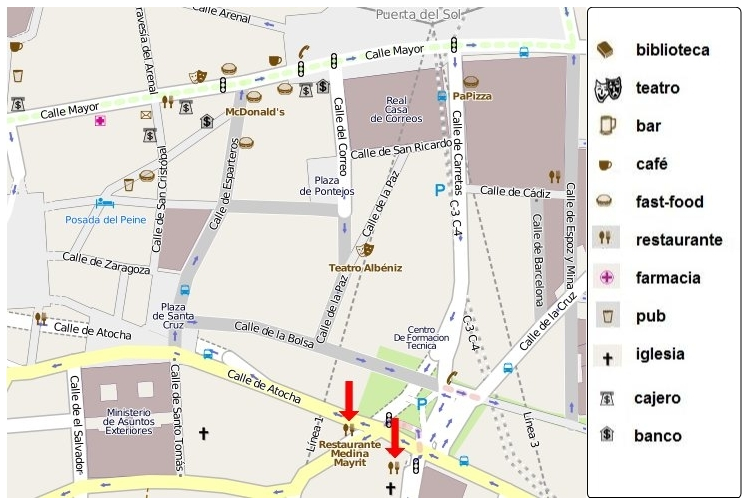
\includegraphics[width=\textwidth]{images/corpus/mapa10.png}\\[0pt]
\caption{Target plural con zoom X}
\label{pluralx}
\end{minipage}
%\vspace*{.1cm}
\begin{minipage}[b]{0.53\linewidth}
\centering
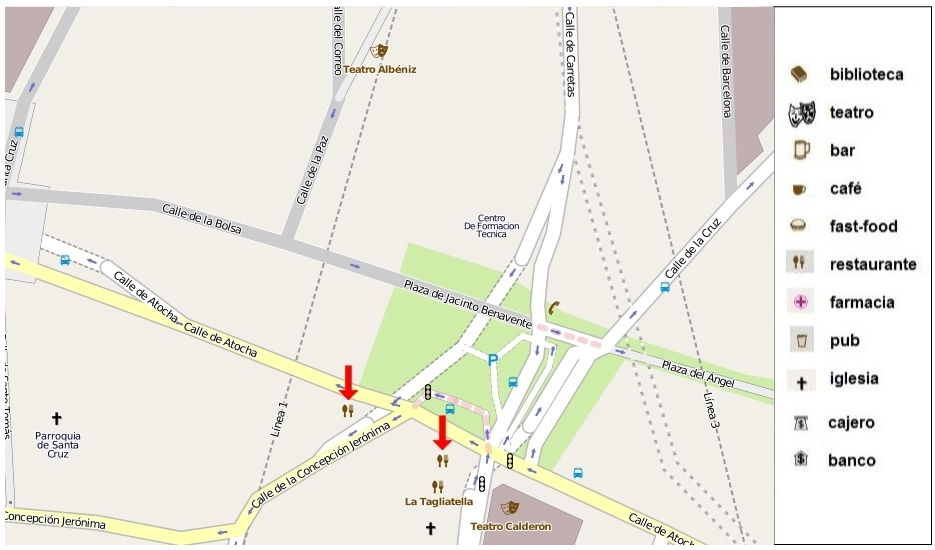
\includegraphics[width=\textwidth]{images/corpus/mapa20.png}\\[0pt]
\caption{Target plural con zoom 2X}
\label{plural2x}
\end{minipage}
\end{figure}
